% This is samplepaper.tex, a sample chapter demonstrating the
% LLNCS macro package for Springer Computer Science proceedings;
% Version 2.21 of 2022/01/12
%
\documentclass[runningheads]{llncs}
%
\usepackage[T1]{fontenc}
% T1 fonts will be used to generate the final print and online PDFs,
% so please use T1 fonts in your manuscript whenever possible.
% Other font encondings may result in incorrect characters.
%
\usepackage{graphicx}
\usepackage{cite}
\usepackage{amsmath, amsfonts, amssymb}
\usepackage{bm}
\usepackage{adjustbox}
\usepackage{amscd}
\usepackage{extarrows}
\usepackage{subfig}
\usepackage{multirow}
\usepackage{eucal}
\usepackage{enumerate}
\usepackage[title]{appendix}

% Used for displaying a sample Figure. If possible, Figure files should
% be included in EPS format.
%
% If you use the hyperref package, please uncomment the following line
% to display URLs in blue roman font according to Springer's eBook style:
% \renewcommand\UrlFont{\color{blue}\rmfamily}

\begin{document}
%
%\title{Empirical Evaluation of Orca 2 Models for Retrieval Augmented Generation}

\title{Evaluation of Orca 2 against other LLMs for Retrieval Augmented Generation}
\titlerunning{Evaluation of Orca 2 against other LLMs for RAG}

\author{Donghao HUANG\inst{1}\orcidID{0009-0005-6767-4872} \and \\
Zhaoxia WANG\thanks{Corresponding Author}\inst{1}\orcidID{0000-0001-7674-5488}}

\authorrunning{D. Huang, Z. Wang}
% First names are abbreviated in the running head.
% If there are more than two authors, 'et al.' is used.
%
\institute{School of Computing and Information Systems, Singapore Management University, 80 Stamford Rd, Singapore 178902, Singapore \\ \texttt{\{dh.huang.2023, zxwang\}@smu.edu.sg}}

%
%\titlerunning{Abbreviated paper title}
% If the paper title is too long for the running head, you can set
% an abbreviated paper title here
%
%Donghao HUANG\inst{1}\orcidID{0009-0005-6767-4872}}
%Zhaoxia WANG\inst{1}\orcidID{0000-0001-7674-5488}}
%
%\authorrunning{Donghao Huang et al.}
% First names are abbreviated in the running head.
% If there are more than two authors, 'et al.' is used.
%
%\institute{School of Computing and Information Systems (SCIS), Singapore Management University (SMU), Singapore \\
%\email{zxwang@smu.edu.sg}\\
%\url{https://www.semanticscholar.org/author/Zhaoxia-Wang/50219296}}
%
\maketitle              % typeset the header of the contribution
%
\begin{abstract}
This study presents a comprehensive evaluation of Microsoft Research's Orca 2, a small yet potent language model, in the context of Retrieval Augmented Generation (RAG). The research involved comparing Orca 2 with other significant models such as Llama-2, GPT-3.5-Turbo, and GPT-4, particularly focusing on its application in RAG. Key metrics, included faithfulness, answer relevance, overall score, and inference speed, were assessed. Experiments conducted on high-specification PCs revealed Orca 2's exceptional performance in generating high quality responses and its efficiency on consumer-grade GPUs, underscoring its potential for scalable RAG applications. This study highlights the pivotal role of smaller, efficient models like Orca 2 in the advancement of conversational AI and their implications for various IT infrastructures. The source codes and datasets of this paper are accessible here\footnote{\url{https://github.com/inflaton/Evaluation-of-Orca-2-for-RAG}}.

\keywords{Large Language Model (LLM) \and Generated Pre-trained Transformer (GPT) \and Retrieval Augmented Generation (RAG) \and  Question Answering \and Model Comparison.}
\end{abstract}

\section{Background and Introduction}
\label{sec:Intro}
In the realm of artificial intelligence, Large Language Models (LLMs) like GPT-4~\cite{achiam2023gpt} have revolutionized how machines understand and process human language. These models, characterized by their vast parameter counts and deep learning capabilities, excel in generating human-like text and comprehending complex language nuances. The emergence of LLMs has opened new avenues in various AI applications, one of which is Retrieval-Augmented Generation (RAG)~\cite{chen2023benchmarking,es2023ragas,lewis2020retrieval,liu2023reta}.

RAG emerges as a promising solution in the quest for enhancing generative tasks, particularly in professional knowledge-based question answering~\cite{es2023ragas,lewis2020retrieval,saad2023ares}. The integration of external knowledge through RAG not only addresses some challenges faced by LLMs, such as hallucination and outdated knowledge, but also facilitates accurate responses in knowledge-intensive tasks~\cite{lewis2020retrieval}. 

The integration of LLMs into RAG systems marks a significant milestone. LLMs enable RAG systems to process and respond to conversational queries with a level of sophistication and relevance previously unattainable. This integration allows for a more intuitive and user-friendly interface, making information retrieval a seamless and interactive experience~\cite{lewis2020retrieval,lin2024revolutionizing}.

While LLMs exhibit impressive capabilities, they often generate fictitious responses~\cite{liu2023reta}. Chen et al. assessed the impact of RAG on LLMs, illuminating challenges and underscoring the need for further advancements in applying RAG to enhance LLM performance~\cite{chen2023benchmarking}. Simultaneously, the role of smaller yet efficient language models, such as Orca 2~\cite{mitra2023orca}, has garnered recent attention. In a landscape dominated by large models, the growing interest in the efficacy of smaller models, particularly in RAG applications, is becoming a notable area of investigation~\cite{mitra2023orca,mukherjee2023orca}.

%% Regarding this RAG, my changes below is ok?
%% i am thinking to delete this paragraph, then change all RAG to RAG. 
%% you decide---
%Extended from RAG, we introduce RAG, an innovative concept that integrates the conversational capabilities of AI with RAG. Unlike conventional search engines that depend on specific keyword queries, RAG systems empower users to communicate in natural, conversational language. This interaction transcends simple query-based exchanges; it encompasses an ongoing, contextually aware dialogue where the system actively participates and comprehends queries within the broader context of the entire conversation.
%%
%%
In this research paper, we delve into the integration of Orca 2~\cite{mitra2023orca}, a groundbreaking smaller language model developed by Microsoft Research, into RAG systems. Orca 2 represents a significant shift in artificial intelligence, characterized by its smaller size but remarkably powerful language processing abilities. This integration promises to significantly enhance RAG systems by offering advanced language understanding and reasoning capabilities with considerably reduced computational demands.

The paper makes the following key contributions:
\begin{enumerate}
     \item[1)] This research provides a comprehensive evaluation of Microsoft Research's Orca 2 in the context of Retrieval Augmented Generation (RAG). This includes a detailed comparison with other significant language models such as Llama-2, GPT-3.5-Turbo, and GPT-4.    
     
    \item[2)] The research assesses key metrics, including faithfulness, answer relevance, overall score, and inference speed. This detailed evaluation aims to provide a nuanced understanding of Orca 2's performance in generating responses within the conversational setting of RAG.
    
    \item[3)] The research underscores the potential of Orca 2 for scalable RAG applications, challenging the conventional belief that larger models are necessary for achieving sophistication in conversational AI. This offers insightful contributions to the field of AI, particularly in understanding Orca 2's role within it.

    \item[4)] The research  positions Orca 2  as a smaller, efficient model that plays a pivotal role in advancing conversational AI. By highlighting its adaptability and performance benefits, the paper contributes to discussions on the evolving landscape of language models and their applications. 
\end{enumerate}
 

%% you can rewrite information below in the "results and discussion/dscovery" section to highligted our discuveries about Orca 2 .

%Orca 2's proficiency in handling complex tasks involving advanced reasoning, even in zero-shot settings, outperforms larger models, making it an ideal candidate for scalable RAG applications. Its adaptability in different environments, especially those with limited computational resources such as mobile devices or edge computing platforms, is particularly noteworthy. Moreover, the model's capability for rapid training and updates aligns perfectly with the dynamic nature of RAG systems, ensuring they stay responsive and relevant to evolving user interactions and data inputs.

%The practical implications of incorporating Orca 2 into RAG systems are vast. It opens up opportunities for deploying more sophisticated, conversational AI systems across various IT infrastructures, without the significant costs and energy demands typically associated with larger models. This integration is not just a testament to the technological advancements in AI but also marks a new era of efficient, accessible, and versatile conversational AI applications.

%The objective of this study was to conduct a comprehensive analysis of Orca 2, exploring its applicability and effectiveness in Retrieval Augmented Generation (RAG) scenarios. Our aim was to offer insightful contributions to the field of AI, particularly in understanding Orca 2's place within it. 


\section{Related Work}
The landscape of language models is rapidly evolving, with advancements in LLMs driving extensive research and exploration of their capabilities across diverse applications~\cite{di2023retrieval}. Notably, GPT-4 has garnered attention for its extensive parameter count and language comprehension capabilities, setting the stage for exploring the potential of smaller yet powerful language models in specific applications~\cite{takagi2023performance}.

Liu et al proposed ChatQA, a family of conversational question-answering models achieving GPT-4 level accuracies through a two-stage instruction tuning method~\cite{liu2024chatqa}. Utilizing a fine-tuned dense retriever on a multi-turn QA dataset, ChatQA-70B outperforms GPT-4 in average score on 10 conversational QA datasets without relying on synthetic data from OpenAI GPT models~\cite{liu2024chatqa}.

RAG represents a promising approach within the field of LLMs, enhancing generative tasks by combining information retrieval and language generation techniques~\cite{es2023ragas,lewis2020retrieval,saad2023ares}. RAG involves retrieving relevant information or passages from documents or knowledge sources and generating responses based on the retrieved content, aiming to enhance the quality and informativeness of generated outputs~\cite{es2023ragas}.

Facing challenges like hallucination and outdated knowledge, LLMs find a potential solution in RAG, which integrates external knowledge, improving accuracy for knowledge-intensive tasks. Gao et al. conducted a comprehensive review exploring the evolution of RAG paradigms, scrutinizing its tripartite foundation, and introducing metrics~\cite{lewis2020retrieval}.

As LLMs and RAG gain prominence in professional knowledge-based question answering, Lin explores the impact of PDF parsing accuracy on RAG effectiveness~\cite{lin2024revolutionizing}. An Automated RAG Evaluation System named ARES utilizes synthetic training data to fine-tune lightweight language models for assessing RAG systems in terms of context relevance, answer faithfulness, and answer relevance~\cite{saad2023ares}. ARES effectively evaluates RAG systems across diverse knowledge-intensive tasks with minimal human annotations, demonstrating accuracy even after domain shifts in queries and documents. 
ARES and Retrieval Augmented Generation Assessment (RAGAS) contribute to the evaluation and assessment of RAG systems, streamlining the process and reducing reliance on human annotations~\cite{saad2023ares,es2023ragas}.

Despite the impressive capabilities of LLMs, they tend to generate fictitious responses~\cite{liu2023reta}. Chen et al evaluated the impact of RAG on LLMs, highlighting the challenges in LLMs and suggesting a need for further advancements in applying RAG to LLMs~\cite{chen2023benchmarking}.

The role of smaller yet efficient language models, like Orca 2~\cite{mitra2023orca}, has been a subject of recent investigation. While large models dominate the scene, the efficacy of smaller models, particularly in RAG applications, is a growing area of interest~\cite{mitra2023orca,mukherjee2023orca}. Microsoft Research's Orca 2 introduces a new paradigm with its smaller size and potent language processing capabilities. This study distinguishes itself by comprehensively evaluating Orca 2's performance against established LLMs in the specific context of RAG, shedding light on its potential contributions to the field.

\section{Methodology}
\label{sec:Method}
\subsection{Workflow Overview}
%RAG leverages pre-trained LLMs through strategic prompting and applying them to contextual private data. Its workflow is usually structured in three distinct phases:

In the assessment of Orca 2 against other LLMs for Retrieval Augmented Generation (RAG), a methodology is employed that involves leveraging various pre-trained LLMs. This is achieved through strategic prompting and the application of these models to contextual private data. As shown in Figure \ref{fig:rag}, the workflow is structured into three distinct phases, ensuring a comprehensive and systematic evaluation process:

\begin{enumerate}
    \item \textbf{Data Preprocessing/Embedding}: This initial phase involves storing private documents, typically PDFs, for later use. The documents are broken down, run through an embedding model, and their embeddings are saved in a vector store.

    \item \textbf{Prompt Construction/Retrieval}: In response to user queries, the system formulates a set of prompts for the language model. These prompts are crafted by merging a template with relevant document extracts from the vector store, with the addition of standalone questions based on existing chat history for enhanced retrieval.

    \item \textbf{Prompt Execution/Inference}: The final stage involves submitting the prepared prompts to a pre-trained language model for processing. This stage utilizes both exclusive model APIs and accessible or in-house models.
\end{enumerate}

\begin{figure}
    \centering
    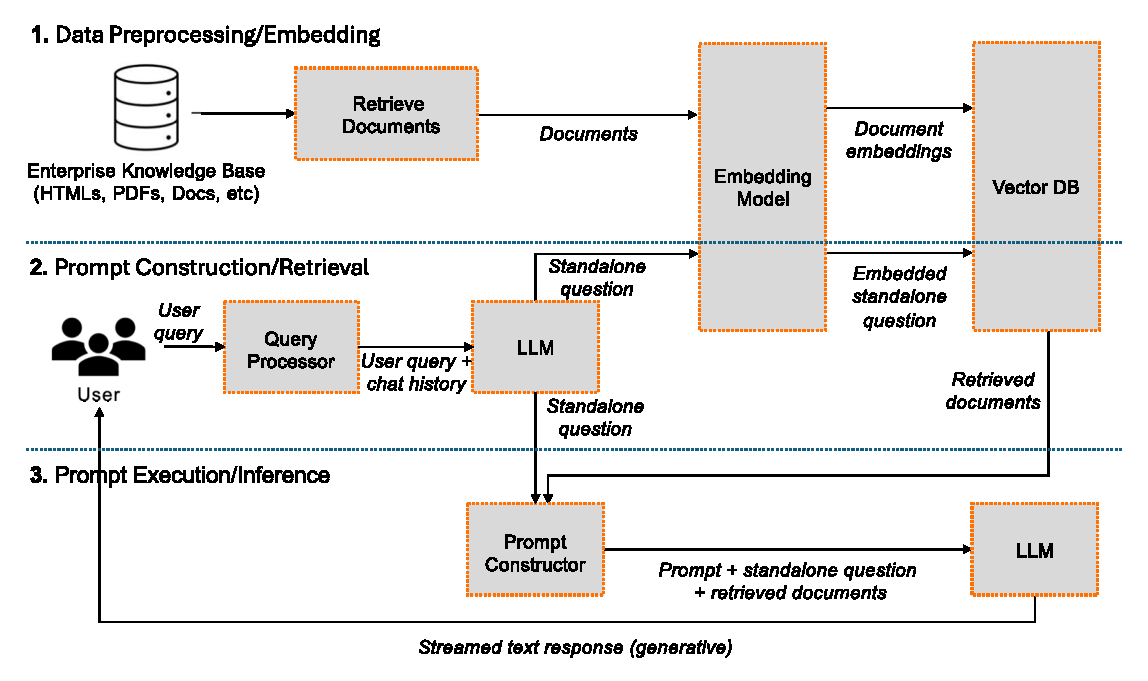
\includegraphics[width=1\linewidth]{figures/RAG.eps}
    \caption{Overall Workflow}
    \label{fig:rag}
\end{figure}

\subsection{Gathering and Processing Data} 
\label{subsec:data}
%We meticulously compiled a dataset from various real-world professional documents, focusing on 13 PDF files related to PCI DSS v4. These files were processed using LangChain framework\footnote{\url{https://github.com/langchain-ai/langchain}} and HuggingFace Instructor\footnote{\url{https://huggingface.co/hkunlp/instructor-large}} for text embedding. The embeddings were stored locally using FAISS\footnote{\url{https://ai.meta.com/tools/faiss}} from Meta for efficient similarity search.

We have carefully curated a dataset from a variety of real-world professional documents pertaining to the Payment Card Industry Data Security Standard (PCI DSS). This standard comprises a comprehensive set of security measures devised by the PCI Security Standards Council to safeguard sensitive payment card information. Our collection process targeted all 13 PDF documents associated with the most recent iteration, PCI DSS version 4.0, released on March 31, 2022, obtained directly from the PCI Security Standards Council's official website\footnote{\url{https://www.pcisecuritystandards.org/document\_library/}}. Subsequently, these documents were processed through text extraction, segmentation, and embedding procedures utilizing the LangChain framework\footnote{\url{https://github.com/langchain-ai/langchain}}  and the HuggingFace Instructor text embedding model\footnote{\url{https://huggingface.co/hkunlp/instructor-large}}, culminating in the generation of embeddings. These were then efficiently stored locally via FAISS\footnote{\url{https://ai.meta.com/tools/faiss}}, an open-source library for vector search created by Meta, facilitating streamlined document retrieval. The complete source code\footnote{\url{https://github.com/inflaton/Evaluation-of-Orca-2-for-RAG/blob/main/ingest.py}} for this procedure is available in our code repository.

%\subsection{Choosing the Models}

\subsection{Assessment and Comparative Evaluation of Orca 2 Against Other LLMs}
In our quest to evaluate the effectiveness of various LLMs for Retrieval Augmented Generation (RAG), we zeroed in on Orca 2 for a detailed analysis. To ensure a comprehensive evaluation, we included comparisons with other prominent models in the field, such as Llama-2, GPT-3.5-Turbo, and GPT-4 from OpenAI. This selection of diverse yet advanced models allows us to conduct a thorough assessment, particularly focusing on how Orca 2's unique attributes and capabilities align with the demands and nuances of RAG applications.

\subsection{Assessment Criteria}
%In our experiments to evaluate LLM's performance in Retrieval Augmented Generation (RAG) contexts, we focused on several key metrics: 

%%must consistent with other sections. if you present this way, you need to draw all the four subfigures in one figure (a,b,c,d)

In our experimental evaluation of Large Language Models (LLMs) for Retrieval Augmented Generation (RAG) applications, our focus are on assessing both Generation Quality and Inference Speed. 

\subsubsection{Generation Quality}
About the Generation Quality, we focused on the key metrics below:

\begin{enumerate}
%    \item \textbf{Faithfulness}: This measures the factual accuracy of the model's responses against the given context. It is calculated based on the consistency of the generated answer with the retrieved context, with values ranging from 0 to 1, where a higher score indicates greater factual accuracy.

    \item \textbf{Faithfulness}: 
    %This metric evaluates the model's responses for factual consistency against the provided context. The evaluation hinges on how well the response aligns with the context provided, with the scoring scale running from 0 to 1—a higher score denotes superior factual alignment. To determine this, we first identify a series of claims within the generated answer. Subsequently, each claim is cross-referenced against the given context to ascertain whether it can be logically derived from it. The formula for calculating the faithfulness score is as follows:
%%I rewrite this portion below
    This metric assesses the model's responses for factual consistency within the provided context. The evaluation is based on how well the response aligns with the context, rated on a scale from 0 to 1, where a higher score indicates better factual alignment.
    To determine the score, we identify a series of claims within the generated answer. Each claim is then cross-referenced against the given context to determine if it can be logically derived from it.

    The formula for calculating the faithfulness score is as follows~\cite{es2023ragas,adams2023meta}: %I add this reference here, right?


\[
    FS = \frac{Number\;of\;contextually\;supported\;claims\;in\;the\;response}{Total\;number\;of\;claims\;in\;the\;response}
\]
where $FS$ represents Faithfulness Score.
    In this process, we employ GPT-4-Turbo to facilitate the identification and verification of claims.
%%I rewrite this portion above. stop here

%    \item \textbf{Answer Relevance}: This metric assesses how pertinent the generated answer is to the given prompt. It evaluates if the response is complete and free from redundant information. Computed using the question and answer, scores range between 0 and 1, with higher scores reflecting better relevance.
    
    \item \textbf{Answer Relevance}: This metric evaluates the relevance of the generated response to the initial prompt. It examines whether the answer is comprehensive and devoid of extraneous information. Scores are calculated on a scale from 0 to 1, based on the question and answer, where higher values denote greater relevance.

    A response is deemed relevant when it addresses the question directly and fittingly. Our relevance assessment emphasizes penalizing answers that are either not exhaustive or that include unnecessary details, rather than assessing factual correctness. To compute this score, the GPT-4-Turbo language model is engaged to generate questions from the given answer multiple times. The mean cosine similarity between these questions and the original question is then measured. The formula for calculating the answer relevance score is as follows\cite{es2023ragas}:
\[
    ARS = \frac{ \sum cosine\_similarity(generated\;question,\;original\;question)}{Number\;of\;generated\;questions}
\]
where $ARS$ represents Answer Relevance Score.    
    This process is predicated on the idea that if the answer adequately addresses the initial question, GPT-4-Turbo should be able to generate questions from the answer that are substantially similar to the original question.
    
%    \item \textbf{Overall Score}: We computed this as the harmonic mean of Faithfulness and Answer Relevance, providing a comprehensive measure of the quality of the generated answers.
    
    \item \textbf{Overall Score}: This metric is the harmonic mean of the faithfulness score and the answer relevance score. It provides a balanced measure of the quality of generated answers, accounting for both the fidelity of the response to factual content and its relevance to the original question. Higher scores indicate better overall performance in producing accurate and relevant answers. The formula for calculating the overall score is as follows:

\[
    Overall\;Score = \frac{2 \times Faithfulness\;Score \times  Answer\;Relevanc\;Score}{Faithfulness\;Score + Answer\;Relevanc\;Score}
\]
    
  %  \item \textbf{Inference Speed}: We also evaluated the models' efficiency by measuring the total number of tokens (words or pieces of words) generated divided by the total inference time. This metric is crucial in real-time applications, as it reflects the model's ability to process and generate responses quickly.
\end{enumerate}
\subsubsection{Inference Speed}
 The Inference Speed of a LLM refers to how quickly the model can process and generate outputs in response to input data or queries. It measures the speed at which the model can make predictions or generate language-based outputs during inference, which is the phase where the model is applied to new, unseen data. A higher inference speed indicates that the model can process information more quickly, making it more efficient for real-time applications and tasks.

%  We also evaluated the models' efficiency by measuring the total number of tokens (words or pieces of words) generated divided by the total inference time. This metric is crucial in real-time applications, as it reflects the model's ability to process and generate responses quickly.

 The formula for calculating the inference speed is as follows:

\[
    IS = \frac{Total\;number\;of\;tokens\;(words\;or\;pieces\;of\;words)\;generated}{Total\;inference\;time}
\]
where $IS$ represents Inference Speed.   
These metrics, especially the first three based on the generation RAGAS\cite{es2023ragas} scores, were essential in comparing Orca 2's performance against other LLMs like Llama-2 and OpenAI models in our RAG scenarios. They provided a detailed assessment of each model's capability in generating accurate, relevant, and timely responses.

\subsection{Experiment Setup}
%Our methodology encompassed a series of meticulously crafted experiments to evaluate the efficacy of Orca 2 in various Retrieval Augmented Generation (RAG) settings. We employed a Python script\footnote{\url{https://github.com/inflaton/Evaluation-of-Orca-2-for-RAG/blob/main/qa\_chain\_test.py}} which was designed to simulate a dialogue between a user and a RAG system, posing the following questions sequentially:

Our study meticulously explored the functionality of Orca 2 across various RAG settings. In assessing the proficiency of LLMs within these RAG scenarios, we crafted a series of inquiries focusing on the PCI DSS standards:

\begin{enumerate}
    \item What's PCI DSS?
    \item Can you summarize the changes made from PCI DSS version 3.2.1 to version 4.0?
    \item new requirements for vulnerability assessments
    \item more on penetration testing
\end{enumerate}

To automate the assessment process, we crafted a specialized Python script designed to simulate conversational interactions with a RAG system. The Python script\footnote{\url{https://github.com/inflaton/Evaluation-of-Orca-2-for-RAG/blob/main/qa\_chain\_test.py}} leverages the LangChain's ConversationalRetrievalChain\footnote{\url{http://tinyurl.com/LCConversationalRetrievalChain}}, a framework designed for generating conversations based on documents that have been retrieved. This particular chain processes the chat history (a series of messages) and incoming queries to produce responses. The operational algorithm of this chain is segmented into three distinct phases:

\begin{enumerate}
    \item It synthesizes a "standalone question" using both the chat history and the new query. If no previous chat history exists, the standalone question remains identical to the new query. If there is existing chat history, however, both the history and the new query are submitted to an LLM, which then generates the standalone question. This method ensures the question is contextually rich enough for effective document retrieval, yet free from unnecessary information that could impede the process.
    \item The formulated standalone question is then fed into a retrieval mechanism. This mechanism employs the Hugging Face Instructor model to create embeddings, followed by utilizing FAISS for a similarity search within the local data storage, as outlined in subsection \ref{subsec:data}, to pinpoint pertinent documents.
    \item Finally, the retrieved documents along with the standalone question are submitted to an LLM, which then generates the conclusive response.
\end{enumerate}

Despite the limitations of a small dataset consisting of only four queries and 13 PDF documents, the study demonstrated the possibility for meticulous system refinement. This underlines the ability of the systems to obtain substantial insights from constrained datasets, showcasing their robustness and adaptability.

To further explore the intricacies of RAG, we developed an interactive, web-based chatbot\footnote{\url{https://github.com/inflaton/Evaluation-of-Orca-2-for-RAG/blob/main/app.py}} using Gradio\footnote{\url{https://github.com/gradio-app/gradio}}, a user-friendly, open-source Python framework for swiftly developing web applications compatible with machine learning models. This chatbot can either be operated on a local machine or hosted on Hugging Face Spaces\footnote{\url{https://huggingface.co/spaces}}, as demonstrated in our own Space\footnote{\url{https://huggingface.co/spaces/inflaton-ai/chat-with-pci-dss}}. Referenced in Figure \ref{fig:hfspace} in the appendix, our chatbot goes beyond basic question-answering functionalities by also revealing the sources from which LLMs derive their responses. Users have the ability to click on the links provided to directly access particular sections of the source documents within PDFs through their web browsers. Furthermore, as outlined in subsection \ref{subsec:data}, we have publicly shared the code for processing PDFs along with this chatbot, thereby providing a comprehensive resource for anyone looking to develop their own RAG-based tools tailored to specific domain data.

\section{Experiments Results}
\label{sec:Results}

The experiments were conducted on a high-specification PC, featuring an NVIDIA® GeForce RTX™ 4090 GPU with 24GB of RAM. Due to the constraints posed by the GPU's memory capacity, it was not feasible to assess the Llama-2-70b model.

\subsection{LLM Generation Quality}
Fig. \ref{fig:perf_scores} presents a comparative analysis of the performance of various Large Language Models (LLMs), including the Orca-2 series and others.

%In the "Faithfulness" section (a), the data illustrates the precision and trustworthiness of each model's information output. All models, except GPT-3.5-Turbo and Llama-2-13b, achieved full marks, showcasing a consistent delivery of faithful results.
In the 'Faithfulness' section depicted in Fig.~\ref{fig:perf_scores} (a), the data illustrates the precision and trustworthiness of each model's information output. Notably, all models, with the exception of GPT-3.5-Turbo and Llama-2-13b, achieved full marks, consistently delivering faithful results.

"Answer Relevancy" shown in  Fig.~\ref{fig:perf_scores} (b) measures the alignment of the models' responses with the queries posed. Vital for application in real-world scenarios, this metric shows Orca-2-13b and Orca-2-7b as top performers, excelling in providing relevant and context-aware answers with scores close to 99\%.

The "Overall Score" calculates the harmonic mean of "Faithfulness" and "Answer Relevancy," offering a stringent performance evaluation. as shown in   Fig.~\ref{fig:perf_scores} (c), Orca-2-13b scores highest, with Orca-2-7b closely behind, indicating a balanced and superior performance.

Collectively, Orca-2 models outshine their Llama-2 counterparts, aligning with the progressive enhancements inherent in the Orca-2 design. The unexpectedly modest performance of OpenAI's models prompts further analysis. To this end, detailed examination of the outputs for specific prompts by all models is documented in Figs. \ref{fig:Question 1} through \ref{fig:Question 4} in the appendix, with standalone questions prominently emphasized to clearly distinguish them from the final answers.

Key observations include:

\begin{enumerate}
    \item In Fig. \ref{fig:Question 2}, both GPT-3.5-Turbo and GPT-4 models struggled to provide answers based on retrieved content, leading to their lower quality scores.


    \item Figs. \ref{fig:Question 2} to \ref{fig:Question 4} reveal an unexpected language switch in the Orca-2-13b model, which starts responding in Spanish after the first question. Despite this, the model maintained high quality scores. This indicates that the RAGAS framework, utilizing GPT-4-Turbo during our experiments, evaluates quality based on semantics, irrespective of the language used. Fig. \ref{fig:translation} in the appendix translates the Spanish content generated by Orca-2-13b, affirming that both the standalone questions and final answers are accurate.

    \item As per Fig. \ref{fig:Question 4}, the Orca-2-7b model generated a generic standalone question, contrasting with other models that produced questions relevant to PCI DSS. Currently, the RAGAS framework lacks a metric to assess the quality of standalone question generation in relation to user input and chat history. Developing such a metric is crucial for enhancing user experience in RAG systems.

\end{enumerate}

These findings underscore the need for continuous refinement in evaluating and enhancing RAG systems, particularly in aspects like language consistency and relevance in question generation. The insights gained from this study contribute to understanding the strengths and limitations of current LLMs in RAG applications.

\subsection{LLM Inference Speed} 
The inference speed comparison among various Large Language Models (LLMs), as depicted in Fig. \ref{fig:speed}, offers significant insights, especially when these models are operated on consumer-grade GPUs. The Orca-2-7b model stands out for its efficiency, achieving an impressive generation speed of around 33 tokens per second. This performance closely matches that of GPT-3.5-Turbo, which generates approximately 32 tokens per second, and significantly outperforms GPT-4's rate of about 16 tokens per second.

A notable observation from the experiments was the slower speeds of 13 billion parameter (13b) models. This reduced performance can be largely attributed to the limitations in GPU RAM of consumer-grade hardware. It was consistently observed that the GPU memory was fully allocated during these tests, which particularly affected the larger models' performance. However, when the Orca-2-13b model was run on a more powerful Nvidia A40 GPU, equipped with 48GB RAM, there was a noticeable improvement, with an average speed increasing to around 15 tokens per second.

This finding highlights the significant impact of hardware specifications on LLM performance and demonstrates the efficiency of smaller models like Orca-2-7b in typical consumer hardware setups. It also indicates that larger models require more advanced hardware with greater memory capacity for optimal performance.

\begin{figure}
    \centering
    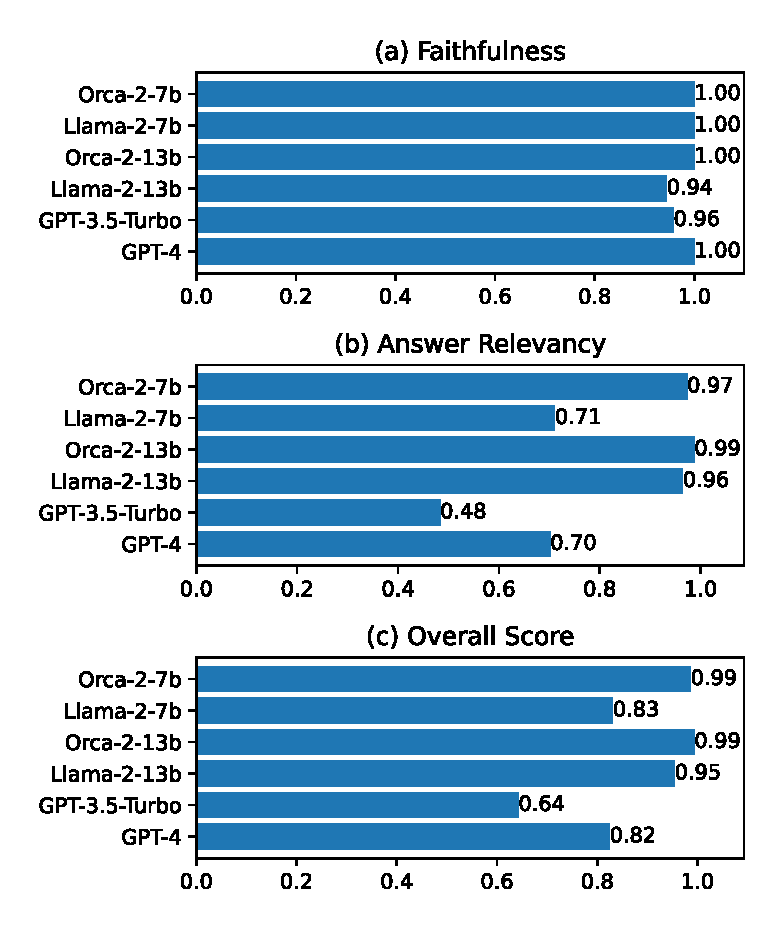
\includegraphics[width=0.6\linewidth]{figures/perf_scores.eps}
    \caption{Comparison of Generation Quality of LLMs}
    \label{fig:perf_scores}
\end{figure}


\begin{figure}
    \centering
    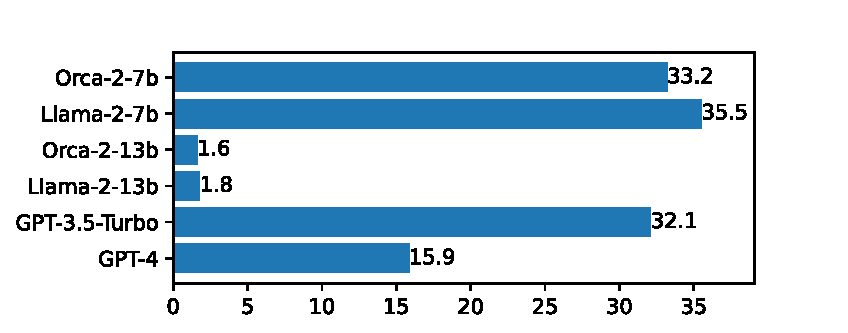
\includegraphics[width=0.6\linewidth]{figures/inference_speed.eps}
    \caption{Comparison of Inference Speed of LLMs}
    \label{fig:speed}
\end{figure}

\section{Conclusions}
\label{sec:Conclusions}
The study conclusively demonstrates Orca 2's superior performance in Retrieval Augmented Generation (RAG), particularly in terms of answer quality and inference speed. Orca 2's ability to generate high-quality, contextually relevant responses rapidly, even on consumer-grade GPUs, sets a new standard in the field. These findings suggest a paradigm shift in conversational AI, where smaller models like Orca 2 can offer efficient, cost-effective solutions without compromising on performance. The study paves the way for broader applications of Orca 2 in various industries, significantly enhancing the accessibility and adaptability of advanced AI technologies in real-world scenarios.

Based on our analysis of Orca 2 within RAG systems, we propose several directions for future research. Firstly, there is a pressing need for advanced evaluation metrics specifically designed for RAG systems, enabling the assessment of contextually relevant standalone question generation—key for enhancing user interactions. Moreover, examining smaller models like Microsoft's Phi-2\footnote{\url{https://www.microsoft.com/en-us/research/blog/phi-2-the-surprising-power-of-small-language-models/}} and Google's Gemma 2B\footnote{\url{https://blog.google/technology/developers/gemma-open-models/}}, noted for their efficiency and compact size, may shed light on the scalability and efficient training of AI models. Investigating the performance of systems like Orca-2 in more complex conversational scenarios, especially those with significant user engagement and larger datasets, remains crucial. This approach will likely improve our understanding of these models' real-world applicability. In subsequent studies, we plan to incorporate additional evaluation tools such as TruLens\footnote{\url{https://github.com/truera/trulens}} and ARES\cite{saad2023ares}, aiming to broaden and diversify our testing methods for a more thorough evaluation across various datasets.

%For future research based on our study of Orca 2 in RAG systems, we propose several key areas of focus. First, there's an evident need for advanced evaluation metrics specifically tailored for RAG systems. These metrics should be capable of assessing the generation of contextually relevant standalone questions, a crucial factor for improving user interactions. Additionally, investigating smaller models like Microsoft's Phi-2\footnote{\url{https://www.microsoft.com/en-us/research/blog/phi-2-the-surprising-power-of-small-language-models/}}, known for its efficiency and smaller parameter size, could provide valuable insights into the scalability and training of efficient AI models. Further exploration into how models like Orca-2 perform in larger, more complex conversational setups, particularly in environments with high user traffic, would also be beneficial. This research direction could significantly enhance our understanding of model applicability in real-world scenarios.

%
% ---- Bibliography ----
%
% BibTeX users should specify bibliography style 'splncs04'.
% References will then be sorted and formatted in the correct style.
%
\bibliographystyle{splncs04}
\bibliography{mybibliography}

%\newpage
\appendix
\section{Appendix}

\begin{figure}
    \centering
    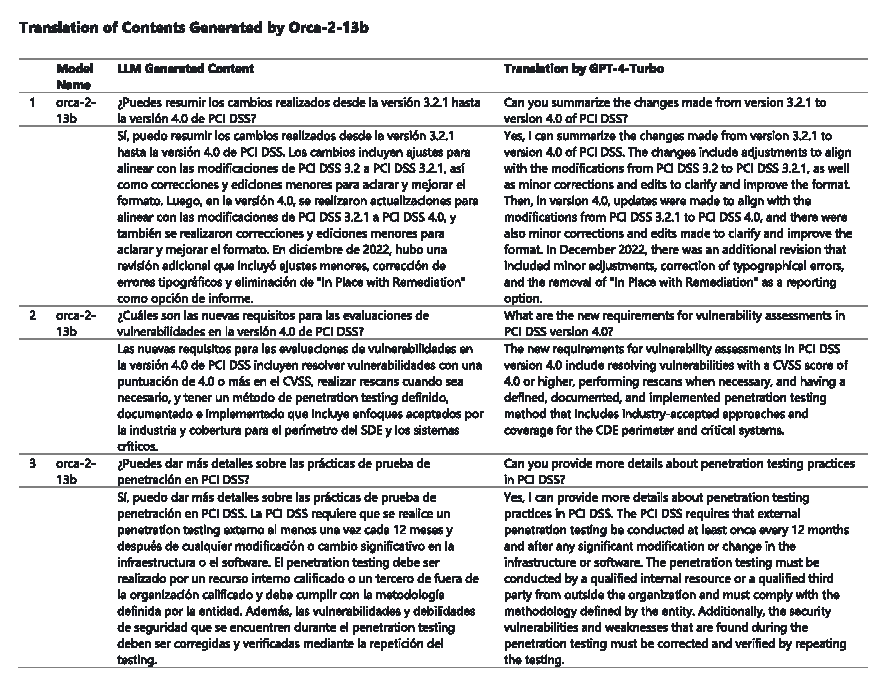
\includegraphics[width=0.9\linewidth]{figures/translation.eps}
    \caption{Translation of Contents Generated by Orca-2-13b}
    \label{fig:translation}
\end{figure}

\begin{figure}
    \centering
    \includegraphics[width=1.3\linewidth]{figures/question_1.eps}
    \caption{LLM Generated Contents for Question 1: What’s PCI DSS?}
    \label{fig:Question  1}
\end{figure}

\begin{figure}
    \centering
    \includegraphics[width=1.3\linewidth]{figures/question_2.eps}
    \caption{LLM Generated Contents for Question 2: Can you summarize the changes made from PCI DSS version 3.2.1 to version 4.0?}
    \label{fig:Question  2}
\end{figure}

\begin{figure}
    \centering
    \includegraphics[width=1.3\linewidth]{figures/question_3.eps}
    \caption{LLM Generated Contents for Question 3: new requirements for vulnerability assessments}
    \label{fig:Question  3}
\end{figure}

\begin{figure}
    \centering
    \includegraphics[width=1.3\linewidth]{figures/question_4.eps}
    \caption{LLM Generated Contents for Question 4: more on penetration testing}
    \label{fig:Question  4}
\end{figure}

\begin{figure}
    \centering
    \includegraphics[width=1.3\linewidth]{figures/hfspace.png}
    \caption{Screenshot of Interactive Chatbot
Web Application Hosted on Hugging Face Spaces Platform}
    \label{fig:hfspace}
\end{figure}


\end{document}